\documentclass[12pt,letterpaper,twoside]{book}
\usepackage{canovel}
\newglossaryentry{foo}{%
  name={FooBar},
  description={A strange animal}
}

\newacronym{nih}{NIH}{Not Invented Here}

\begin{document}

\graphicspath{
  {"assets/images/"}
  {"../assets/images/"}
}

% book title page
\title{Computer Science \\
  \large The Novel}

\author{Roie R. Black}



\frontmatter
\maketitle

% table of contents
\renewcommand\contentsname{Table of Contents} % rename title
\tableofcontents
\chapter*{Preface}
\addcontentsline{toc}{chapter}{Preface}

For almost two decades, I taught a course titled \emph{Computer Architecture
and Machine Language}. The course was offered to second year college students
intending to become computer scientists. This course was by far my favorite
one, since it let me take students on an exciting journey of discovery.

When I first was offered this course, the basic material covered assembly
language programming for the Intel 8086 processor. Architecture took a back
seat to learning another programming language. I found that odd that the course
focused on a 16-bit processor since most computers at the time were using
32-bit Pentium processors. Upgrading the course required new development tools,
and I decided to make the course vendor neutral. That meant getting rid of the
Microsoft bias present in many courses at my school. I started off by deciding
to introduce my students to tools commonly found in open-source projects. Those
tools included programmer's editors, build tools, source code control tools,
and standards compliant compilers capable of building projects on any platform.
Many of my students were shocked to learn that they could build software
without using some magical \emph{Integrated Development Environment}. My theory
was simple. Choosing an IDE is something best left to that first job the
student will land. That job will have an development process and tool chain
that the new employee will need to learn. 

As the course evolved, I added more emphasis on the inner workings of the
machine the students were learning to program. At first the focus was still on
Intel chips since they power most of the computers students are familiar with.
However, the world is changing, and more and more work is being done on systems
that use other processors. The most common chips in mobile platforms today are
variants of the \emph{ARM} processor. 

The \emph{ARM} processors are complex chips, maybe too complex for beginners in
my course to study. There was a simple alternative available though. The
\emph{Microchip AVR} processor found on the new |emph{Arduino} development
boards was available very inexpensively. I decided to buy enough of these
boards to set up lab kits for my classes so students could do hands-on
development work on real hardware.

The course became very popular. It was challenging, but prepared students well
for their future jobs.

I continues to add material focusing on what was going on inside the processors
they were learning to control. Then in 2017 something interesting happened. The
Texas body charged with setting standards for college courses changed the
course requirements for my course in an interesting way. The new guidelines
asked students to write a simulator for a real processor as part of the course.
They also added a focus on embedded processors intending to get students ready
for those mobile platforms found everywhere. I was already doing most of what
they asked. I only needed to add the simulator to my course to meet these new
guidelines.

This book is designed for this course. Although I have now retired, I decided
to write this book based on my lecture notes but with a new twist.

Instead of producing yet another dry textbook, I decided to write a book along
the lines of one of my favorite books: \emph{Godel, Escher, Bach} by Douglas
Hofstadter \cite{Hofstadter:1999}. The result is not so much a textbook, but more
of a novel. I want the student to want to read this text, not just scan it
looking for answers to exercises they are given. I hope the result is
interesting enough to show them why they are learning all this new material. I
also hope to produce more professional candidates for that job market waiting
for them in their near future.

I hope you enjoy reading this book as much as I enjoyed producing it.

Roie R. Black \\
Major, USAF (retired) \\
Professor, Computer Science (retired) \\
Austin Community College, Austin, Texas


\cleardoublepage
% \phantomsection
\addcontentsline{toc}{chapter}{\listfigurename}
\listoffigures
\listoftables

\mainmatter
\chapter{Blue Flames}

In a quitet basement somewhere in Dayton, Ohio, two young students are working
into the night on a computer. No, this is not a fancy desktop or laptop
computer. It is a simple machine designed to help one of the students learn how
to program in assembly language.

Ada is the student who is building the computer, and her friend, Alan, is
helping her get the critter running. Ada has managed to come up with a nice case
for her machine. The sides of the case are cherry wood which she will finish
off later to make things look nice. The actual case is a bent piece of aluminum
sheet metal she convinced a local automotive body shop to fabricate for her.

The goal this evening is to power the gadget up. Alan is working on wiring a
power supply for the machine that will be bolted inside the case. A switch will
be attached to the sheet metal cabinet along with a keypad and an LED display. 

Ada is bolting a small printed circuit board to the bottom of the case. This
board comprises a complete 8-bit computer system. It is not fancy, nor is it
very powerful, but it will be sufficient for Ada's goal. Alan is wiring up the
power supply and the switch. Both of them work together to get everything
installed in the case, ready for the first power-up!

The evening wears on, and things are getting close to ready. Another student,
Nick, wanders down the stairs into the basement.

"Hey Ada, have you got the thing powered up yet?"

"Just about. Alan is almost finished with the power supply."

Alan puts a screwdriver down on the table.

"Ready for the first test. Ada, you do the honors!"

Ada reaches a nervous hand toward the switch. All three of them hold their
breath. Ada flips the switch.

A brief flash of light is seen inside the case, and the lights go out!

In the darkness, Nick mutters "I guess you flunked the Blue Flame test!"


\chapter{Atoms}
\section{What is an atom?}
If we take anything physical in our world, and start tearing it down into
smaller and smaller chunks, eventually we end up looking at a structure we call
an "atom"\index{atom}. For a long time, humans resisted the idea that there was such a
gadget, today, we put a lot of energy into researching what happens if we tear
and atom apart to see what it is made up of. We even want to go a bit further and
see what those atomic parts are made up of.

Welcome to the world of high-tech physics!

We will not dive smaller than the basic atom. (Real, serious physicists are
trying to go much farther!) That will let us look at its most basic parts.

Some of this, you should have learned in your high school chemistry class!

\subsection{Basic Atom Structure}
An atom is sort of like a tiny solar system. There is something big in the
center of this system, and a bunch of smaller things flying around that center
in tiny orbits.

\begin{figure}[ht]
  \caption{The Atom.}
  \centering
  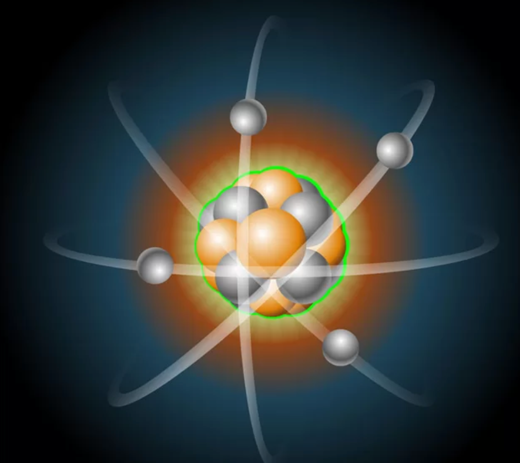
\includegraphics[width=.6\textwidth]{atomic-structure.png}
\end{figure}

Atoms are pretty small. Estimates as to their size depends on the material, but
a single atom is as small as $10^{-8}cm$ in size. That is pretty small.
But, amazing as it might seem, we can build machines that can move single
atoms. Take a look at this image, created by IBM engineers in 1989. The image
was taken using a scanning electronic microscope!

\begin{figure}[ht]
  \caption{IBM's atomic logo.}
  \centering
  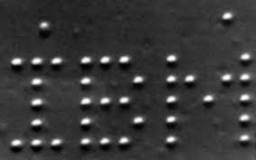
\includegraphics[width=.6\textwidth]{IBMlogo.jpg}
\end{figure}

Those bumps are actually single atoms, nudged into place to create this logo.
Amazing!

\subsubsection{Electrons}

The particles flying around the center are electrons. \index{Electrons} These particles are
tiny! Linus Pauling, a Chemist who won the Nobel Prize for Chemistry in 1954,
thought they were on the order of $< 10^{-18}cm$ in size. That is pretty
small.

These electrons carry a charge (actually a negative charge). 

..  note::

    Contrary to popular thinking, if something is positively charged, that
    means it has fewer electrons than it wants to have. If something is
    negatively charged it has too many electrons than it wants to have.
    Electrons are attracted to positively charged things, and repelled
    by other negatively charged things.

    So, two electrons hate each other, and want to keep away from each
    other.

\subsubsection{Protons}

At the center of our tiny solar system sits a clump called the core. This
core is made up of two more tiny elementary particles. One is the
proton.

Protons are about $10^{-13}$ cm in size. That is
(1000 times bigger than an electron!)

Protons carry a positive charge. In a single atom, there should be as
many protons as there are electrons flying around this atomic core. 

As long as this is true, the atom is happy, and the electrons sit there, flying
around the core with its pile of protons.

\subsubsection{Neutrons}

The second particle in the core is called a neutron, which carries no
charge. Neutrons are about the same size as protons. Neutrons are
not attracted to either electrons or protons. They just sit there,
stuck to the protons in that core. What they do is give the atom addition
mass (think weight).

\section{Atomic Numbers}

We like to classify things. At the level of atoms, we assign an atomic
number to each kind of atom we discover. Those protons and neutrons
in the core both act in a similar way. So we lump them together and call
then neucleons. The ``atomic number is the number of neucleons in the
atom. (Where do you think the term nuclear physics came from?)

\subsubsection{Ions}

Since electrons are always flying around, and the core just sits there,
there is the possibility that an electron will get close enough to another atom
that it will fly off of the first atom, and join in the mess of electrons
flying around the second atom. The atom that the electron left is now left
with more protons than electrons and has a net positive charge. It
is not happy in this state, but there is not much it can do. The second atom is
also "unbalanced". It has more electrons than protons and has a net
negative charge. That second atom is also unhappy. We call these "unhappy"
atoms ions. 

..  note::

    We have names for each kind of ion. A positively charged ion is
    called an cation, and a negatively charged ion is called an
    anion. Cations are also called "metals", and an anion` is called a
    "non-metal". The terms anode and cathode refer to points in a
    device where the charge is more positive, or more negative. Makes sense,
    right?


We can create ions by heating atoms up and firing a stream of electrons
at them. Those electrons can knock off other electrons from each atom, setting
up this ionized state. The mess at the middle of this action is called a
plasma, and it has interesting properties, but we will not explore them
here. Plasmas might be interesting if you need to wipe out space aliens!

\subsubsection{Stable Ions}

Some ions are content with being "unbalanced", but only up to some limit.

For example Sodium is an element with 11 protons in the core, and 11
electrons spinning around. It is happy in this normal state. But, Sodium
will tolerate losing an electron, becoming a Sodium ion. The chemical symbol
for Sodium is $Na$ and the term for the Sodium ion is $Na^{+}$. This
ion is positively charged).

Chlorine is another element, this one with 17 protons, and 17
electrons. Chlorine is happy to accept another electron, becoming a
Chloride ion. The chemical symbol for Chlorine is $Cl$. The Chloride ion is
$$Cl^{-}$$. It is negatively charged.

When these two ions get near each other, they "bond". The electron does not
move from one to the other, but the attractive force causes them to move close
together.  This "bond" is pretty strong, and the result is a lattice of atoms we
call a crystal. This one is known as "salt"! The chemical symbol for this
is $$NaCl$$. The original ions are still ions, but they are quite happy being
close together.

\subsubsection{Metals}

We already mentioned the term metal. That term describes an element with a
strong willingness to lose an electron, becoming a cation. When many of
these atoms get together in a material like copper, they collectively let
electrons fly off, forming a sea of electrons that fly around, seemingly at
random, surrounding the entire collection of atoms. These electrons are called
free-electrons because they have no real home on any single atom. This sea
of electrons produces something called conductivity, a willingness of a
material to let electrons move easily. New electrons can join into this
sea, others can be pulled off.

\section{Electric Fields}

An electric field is a region around an charged particle. The charge at any
point in that area around the charge is measured in something we call
volts. Voltage is a measure of the electrostatic potential energy
available at that point. Near a positive charge, the voltage is high, near a
negatively charged particle it is low. 

It takes energy to move a point from one voltage to another one. It takes a lot
of energy to move a voltage higher, just as it takes energy to lift an object
to a higher position above the ground. Once at the high point there is a
potential to release that energy by moving the object (or the charge) to a
lower point. 

The strength of this electric field is measured in something we call volts.

When electrons move, they generate a magnetic field around them, often called
an electromagnetic field, since there is a magnetic field and an electric
field at work at the same time. All of this is described by Maxwell's
Equations, which are the foundation of many technical disciplines, especially
radio. Those waves propagate through space, interact with other metals, and
induce electrons to move in those metals. (Hey, that is how radio works!)

\subsection{Electricity}

We now have enough background to explain how electricity works (well at least
in a (very) simple way!)

I have a cool book called \emph{There are no Electrons, Electronics for Earthlings} \cite{Amdahl:1991}. In
that book the author describes electrons as "party animals" who need to party.
The parties are all at positively charged points. The electrons are attracted to
those parties, and work tirelessly to find their way to them! However, they
must travel over "conductive" paths. Something like a copper wire will do
nicely!

\subsubsection{Batteries}

There has to be a source of both positive and negative charges in any
electrical system. That source is often called a ``battery``. The battery is a
device that can hold both positive and negatively charged particles, but it
separates them with a wall, preventing them from getting together. Instead, the
battery has two terminals, One will let electrons loose, the other is where the
party is.

Now, if we provide a path from the electrons to the party, those electrons will
fly. Actually a stream of electrons will join the sea of free electrons in the
mtal, and that will cause many of them to seem to move toward the other end.
The path is called a "circuit".

..  warning::

    It is vitally important that we not allow all the electrons to the party at
    once. That can cause very harmful side effects, like smoke! That is called
    a "Short Circuit". Batteries have been known to explode if this happens!

    Usually, we put some gadget in the circuit that slows things down. A light
    bulb will do. The bulb is designed so that it slows the electrons down.
    They want to move, so they get hot. The heat produces light. Cool! (Well,
    actually, HOT!)


\section{Who Cares?}

This is a computer architecture text, What does this have to do with
Computers?

Well, think about this simple C++ code fragment:

\begin{minted}[linenos,frame=lines,framesep=2mm]{c++}
int main(void) {
    int x, y=5;
    x = y;
}
\end{minted}

What needs to happen to make this statement work? How do you think the
computer is going to make this actually happen? The answer is simple. It will
launch some of those party animals, and cause them to travel from the place
called "y" to the party at the place called x". We design a machine that
causes the electrons to carry "data" along as they move to the party!

Wow!

Now, don't panic. You do not need to understand all of the physics in this
discussion. It will not appear on a test. 

I, on the other hand, and one of those crazy folks who keeps digging, as far
down as I can go. It gets more fascinating as you dig deeper. 

..  warning::

    You can kill a lot of time Googling all of this! You have been warned!














\chapter{Nick's Lab}

Nestled near a fence behind Nick's home sits a small wood frame building. The
building is old enough that it must have been there before the nearby home was even 
built.  Inside of this building are several wooden workbenches filled with equipment
used to study electricity. The test gear is surrounded by a sea of wires. 

On the back wall of the building is a small window that opens up to the pasture
on the other side of the fence. Several Arabian horses spend their days in that
pasture, and occasionally wander up to see what is goin on inside of the
building. 

This is Nick's lab. When he is not studying for school, Nick spends a lot of
time in this lab playing with electricity and trying to figure out what it can do.
Nick keeps a supply of carrots handy when he works, and when a horse sticks its
head in the window, a carrot is usually delivered to keep him happy.

Nick has run electrcity to this building from his home so he can work on his experements.
Nick has always been fascinated by Eelectricity. When he was a kid, he took some wire, a
light buld and a battery and built a simple flashlight. That silly gadget was
used to read magazines under the covers in his room when he was supposed to be
sleeping.

Seated in Nick's lab is the last member of our gang of students. Leo is tearing
apart an old radio to see what makes it work. The radio dates back to the 1940s
and Leo's grandfather told him he used it to listen to the BBC during World War
II. The radio was sitting unused in an upstairs room in his grandfather's
house. Two wires were running from the back of the radio out a nearby window.
One of the wires extended up into a tree some distance from the house. The
other wire ran down the side of the house and was connected to a water pipe
that went into the ground. Leo had to disconnect those wires before he took the
radio to Nick's lab for proper study.

\includegraphics[width=0.6\textwidth]{his020r.jpg}

Leo is one of those strange people who loves to take things apart. Sometimes he
even manages to put them back together again. The back of the radio is made os
some kind of wood his grandfather called bakelite. Leo removed the five screws
holding the bakelite panel in place so he could see what was inside. Then he
plugged the radio into the wall socket and turned the knob on the front of the
radio. That knob was supposed to power up the radio and adjust the volume
according to his grandfather.

Leo was not quite sure what to expect, but looking inside he saw a set of seven
glass gadgets all of which were glowing and giving off quite a bit of heat. "This is
crazy" Leo muttered to himself!

There was nothing coming out of the radio. That might be because Leo had not
hooked up those two wires. Maybe those were needed to make it really work
properly.

The rest of the gang arrived as Leo was pondering the glow inside of his radio.
Alan piped up first.

"Hey Leo, I see you have managed to light up some old vacuum tubes! Those were
common when dinosaurs roamed the Earth."

"Funny, Alan. I just want to understand how this old thing manages to produce
sound."

"You really need to attach an antenna to that thing" was Nick's comment. 

Leo was still puzzled. "But how does a wire sitting up in the sky manage to
make the radio work?".

"Electromagnetic waves induce a current in the wire which the radio processes
into sound."

Ada chimes in. "Leave it to Alan to speak in tounges that mean nothing to the
rest of us! I guess we all have tome studying to do"

Nick has other ideas in mind.

"I thought we were here to see some real sparks fly."

"Fine, as long as we do not get burned by anything." Ada was just being a bit
cautious. All these folks knew they were immortal, at least until they reached
35 years old! Still, it never hurts to be careful, especially in Nick's lab!

Nick walks over to another workbench. Sitting in the middle of this bench is a
cardboad tube about a foot long with thin wire wound around it from top to
bottom. At the bottom of this tube is another coil of wire attached to some
electronic gadgets and finally attached to a power supply plugged into the
wall. At the top of the long tube is a silver donut made out of aluminum. 

"Leo, hit the lights!"

Nick flips the switch and sparks several inches lone shoot out of the donut,
dancing in the air. The smel of ozone fills the room.

"That is definitely way cooler than Alan's miswired switch!" says Ada.

Leo is intrigued. "It looks like electricity zooming through those wires
managed to generate something that made lightning fly away from that donut. Did
the coil make that happen?"

Alan contributes more of his vast wisdom. "When you make electricity move
around in circles like that, an electromagnetic wave is produced that moves
away from the coil. What is really cool is what happens if you hold a
flourescent light near this coil. It lights up with no connections. Somehow
that electromagnetic wave gets turned back inot enough electricity to light the
bulb."

Aha! That is the basis of radio!" Leo has figured out why the antenna wire is
needed to produce any sound. "But what is the other wire all about? The one
connected to the water pipe."

\makeatletter
\def\input@path{{../}}
\makeatother
\documentclass[../main.tex]{subfiles}

\begin{document}
\chapter{Bibliography}
\bibliographystyle{plain}
\bibliography{references}
\end{document}


\printglossary[type=\acronymtype,title={List of Abbreviations}]
\begin{appendix}
\documentclass[../main.tex]{subfiles}
\begin{document}
\chapter{Appendices}
\end{document}


\chapter{Cast of Characters}

I want my text to be something you want to read. In today's hurry-up
world, students actually do not read as much as they did in the past. That is
sad, because you can learn a lot from reading a well-written text.

Yes, there are badly written textbooks around, maybe even mine!

Probably, my most favorite book is \it{Godel, Escher, Bach}, by Douglas Hofstader
\cite{Hofstadter:1999}. I first read this, shortly after it came out. In this
book a set of characters lay out an interesting concept in one short chapter,
then the next chapter presents that concept in terms that are now fun to read.
The normally dry text, suddenly comes to life. Douglas won a Pulitzer Prize for
this book, As a Computer Science student, you should read it! I am currently on
my seventh pass through it!

I am stealing Douglas' idea, I have my own characters, and I will use them in
these notes on occasion.

We will follow four characters through our journey into computers and
programming. These four are good friends, but have very different goals in
life. That affects how they approach problems they encounter.

Like all teams, they have to work through their differences and come up with an
approach to getting some job done that works for everyone.

Here are our characters:

* Nick:   The "Doer"

..  image:: nikola-tesla.jpg
    :align: center
    :width: 200

Nick has a few interesting characteristics:

    * Tank - impervious to harm. 

    * Gets blown up a lot, but survives
    
    * Hates to wait for anything
    
    * Needs lots of documentation
    
    * Can fix anything
    
    * Mechanical genius

    * Drives a Ford Mustang (GT)

    * Uses Windows 10 Pro

    * named after: `Nikola Tesla`_
    

* Ada:  Curious about everything!

..  image:: ada-lovelace.jpg
    :align: center
    :width: 200

Ada is going to learn as much as she can about everything. She has a burning
desire to know something about everything!

    * Questions things a lot

    * Never quit asking "why" when told how something works.

    * Tends to stop working on a problem when she sees the answer

    * Seems interested in everything, especially technical stuff

    * She is a peace maker, trying to calm things down when they get tense.

    * Drives a Prius

    * Uses a Macbook Pro

    * Named after `Ada Lovelace`_

* Leo

..  image:: leorardo-da-vinci.png
    :align: center
    :width: 200

Leo is the mechanic of the bunch. He is constantly taking things apart so he
can figure out how they work. He is also an artist. As he disassembles things,
he makes drawings of the gadgets he is studying. Leo can take a box of junk and
come up with a Ferrari!

    * He can see how things move, because he understands how they are put together.

    * Likes to concoct new machines.

    * Rube Goldberg is his idol!

    * Drives a 1964 Alfa Romeo Giulia Spider sports car.

    * He does not own a stinking computer!

    * Named after `Leonardo da Vinci`_
* Alan

..  image:: alan-turing.jpg
    :align: center
    :width: 200

Alan is the genius of the group. He does know a lot about everything. In fact,
tripping him up is a game the other two like to play. How he got this way is a
puzzle, but he has been caught, late at night, scouring the Internet with his
iPad!

    * comes across al very knowledgeable, even if he is not really that up on
      something.

    * Has a photographic memory, seldom forgets anything

    * Wants to guide the action because he knows the "right way"

    * Something of a space cadet, he wanders off track at times

    * Drives a Mercedes (he got it used)

    * Uses Linux on an Alienware Laptop

    * Named after `Alan Turing`_

..  _Alan Turing:    https://en.wikipedia.org/wiki/Alan_Turing
..  _Ada Lovelace: https://en.wikipedia.org/wiki/Ada_Lovelace
..  _Nikola Tesla: https://en.wikipedia.org/wiki/Nikola_Tesla
..  _Leorardo da Vinci: https://en.wikipedia.org/wiki/Leonardo_da_Vinci
..  _Rube Goldberg: https://en.wikipedia.org/wiki/Rube_Goldberg

\end{appendix}

\printglossary

\end{document}

